% !TeX root = ./main.tex
\documentclass[main]{subfiles}
\begin{document}
\part*{Дифференциальная геометрия}
\chapter{Дифференциальная геометрия кривых}
\section{Понятие кривой} \marginpar{05.09.22}
Кривую можно задать множеством способов, например:
\begin{itemize}
    \item в декартовых координатах: $y = f(x)$
    \item в полярных координатах: $r = r(\phi)$
    \item неявным уравнением: $F(x,y) = 0$
\end{itemize}
но обычно её задают в параметрическом виде:
\[\begin{cases}
        x = x(t) \\
        y = y(t) \\
        z = z(t)
    \end{cases}\]
В таком случае кривая
\begin{itemize}
    \item в декартовых координатах принимает вид: $\displaystyle\begin{cases}
                  x = t \\
                  y = f(t)
              \end{cases}$
    \item в полярных координатах: $\displaystyle \begin{cases}
                  x = r(t) \cos t \\
                  y = r(t) \sin t
              \end{cases}$
    \item для неявных уравнений свои методы, т.к. не очень понятно как с ними работать
\end{itemize}

Например, для неявных уравнений существует следующая теорема:
\begin{theorem*}[О неявной функции]
    Если $F(x,y) = 0$ и $F(x_0, y_0) = 0$,
    а так же $\frac{\partial F}{\partial y}\rvert_{(x_0, y_0)} \neq 0$,
    $\frac{\partial F}{\partial x}, \frac{\partial F}{\partial y}$ существуют и непрерывны в окрестности $(x_0, y_0)$,
    тогда существует $f(x)$ в некоторой окрестности $x_0$, что $F(x, f(x)) =0$.
\end{theorem*}
\begin{example}
    Имеем стандартное уравнение окружности: $x^2 + y^2 -1 =0$.
    В окрестности большинства его точек можно выразить $y$ через $x$: $y = \pm \sqrt{1-x^2}$.
    Но это выражение перестает работать в точке $x=-1$ или $x=1$
    (то есть для любой другой точки, можно найти окрестность, такую что функция будет иметь конкретный знак, в то время как для $x= \pm 1$ такое сделать невозможно).
    Воспользуется теоремой выше, соблюдены почти все условия, кроме:
    \[\frac{\partial F}{\partial y} = 2y\rvert_{\substack{x = \pm 1\\ y=0}} = 0\]
    Соответственно, именно в этих точках найти искомую $f$ нельзя.
\end{example}

\subsection{Параметрическое задание кривой}
$\vf (t)$ - векторное уравнение. $\vf: [a,b] \to \R^3$.
Кривую определяет вектор-функция.

\begin{definition}[Вектор-функция]
    $\vf$ -- вектор-функция как выше.
    На протяжении всего курса предполагаем, что у функции необходимая нам гладкость.
\end{definition}

\begin{definition}[Предел вектор-функции]
    $\displaystyle \lim_{t \to t_0} \vf (t) = \vv$, если
    \[\forall \epsilon > 0 \ \exists \delta > 0 \ |t - t_0| < \delta \ |\vf(t) - \vv| < \epsilon\]
\end{definition}
\begin{propertylist}
    Везде считаем, что свойство выполнено, если существуют соответствующие пределы.
    \begin{enumerate}
        \item $\displaystyle \lim_{t \to t_0} ( \vf(t) \pm \vg (t))= \lim_{t \to t_0} \vf(t) \pm \lim_{t \to t_0} \vg (t) $
        \item $\displaystyle \lim_{t \to t_0} ( \vf(t) \vg (t))= \lim_{t \to t_0} \vf(t) \lim_{t \to t_0} \vg (t) $
        \item $\displaystyle \lim_{t \to t_0} ( \vf(t) \times \vg (t))= \lim_{t \to t_0} \vf(t) \times \lim_{t \to t_0} \vg (t) $
        \item Смешанное произведение аналогично
    \end{enumerate}
\end{propertylist}

\begin{definition}[Производная вектор-функции]
    \[\vf'(t)\rvert_{t=t_0} =  \lim_{t \to t_0} \frac{\vf(t) - \vf(t_0)}{t - t_0}\]
\end{definition}

\begin{propertylist}
    \

    \begin{enumerate}
        \item $\displaystyle (\vf \pm \vg)' = \vf' \pm \vg'$
        \item $\displaystyle (c\vf)' = c\vf'$
        \item $\displaystyle (\vf \vg)' = \vf'\vg + \vf \vg'$
        \item $\displaystyle (\vf \times \vg)' = \vf' \times \vg + \vf \times \vg'$
              \begin{proof}
                  \begin{multline*}
                      (\vf \times \vg)'\rvert_{t=t_0} = \lim_{t \to t_0} \frac{\vf(t) \times \vg(t) - \vf(t_0) \times \vg(t_0)}{t - t_0} = \\
                      \lim_{t \to t_0} \frac{\vf(t) \times \vg(t) - \vf(t_0) \times \vg(t) + \vf(t_0) \times \vg(t) - \vf(t_0) \times \vg(t_0)}{t - t_0} = \\
                      \lim_{t \to t_0} \frac{\vf(t) - \vf(t_0)}{t - t_0} \times \vg(t) + \lim_{t \to t_0} \vf(t_0) \times \frac{\vg(t) - \vg(t_0)}{t- t_0} = \\
                      \vf'(t_0) \times \vg(t_0) + \vf(t_0) \times \vg'(t_0)
                  \end{multline*}
              \end{proof}
        \item $\displaystyle (\vf,\vg,\vh)' = (\vf',\vg,\vh) + (\vf,\vg',\vh) + (\vf,\vg,\vh')$
              \begin{proof}
                  \begin{multline*}
                      (\vf,\vg,\vh)' = ((\vf \times \vg) \vh)' = (\vf \times \vg)' \vh + (\vf \times \vg) \vh'=\\
                      (\vf' \times \vg) \vh + (\vf \times \vg') \vh + (\vf \times \vg) \vh'
                  \end{multline*}
              \end{proof}
    \end{enumerate}
\end{propertylist}

В свойствах отсутствует деление, т.к. операция деления векторов не определена.
В вещественном анализе множество теорем доказывается с помощью следующей теоремы:
\begin{theorem*}[Лагранжа]
    Если $f(x)$ непрерывно дифференцируема на $[a,b]$, тогда существует $c \in [a,b] : f'(c) = \frac{f(b) - f(a)}{b-a}$.
\end{theorem*}
Для вектор-функций эта теорема, однако, не существует!


\begin{definition}[Интеграл вектор-функции]
    \[\int_a^b \vf(t) dt = \lim_{\max |\Delta_i t| \to 0} \sum_i \vf(\sigma_i) \Delta_i t.\]
\end{definition}
\begin{definition}[Кривая]
    Кривая -- образ $\vf(t)$.
    Кривая не пересекает саму себя, то есть $\vf(t_1) \neq \vf(t_2)$.
    $\vf(t)$ -- параметризация кривой.
    Параметризация регулярна, если $\vf'(t) \neq \vzero\ \forall t$.
\end{definition}
\begin{example}[Нерегулярная параметризация]
    $\displaystyle \begin{cases}
            x = t^2 \\
            y = t^3
        \end{cases}$ или $\vr(t) = (t^2, t^3)$ --
    полукубическая парабола. $y = x^{3/2}$ (плохо при $x<0$).
    \begin{center}
        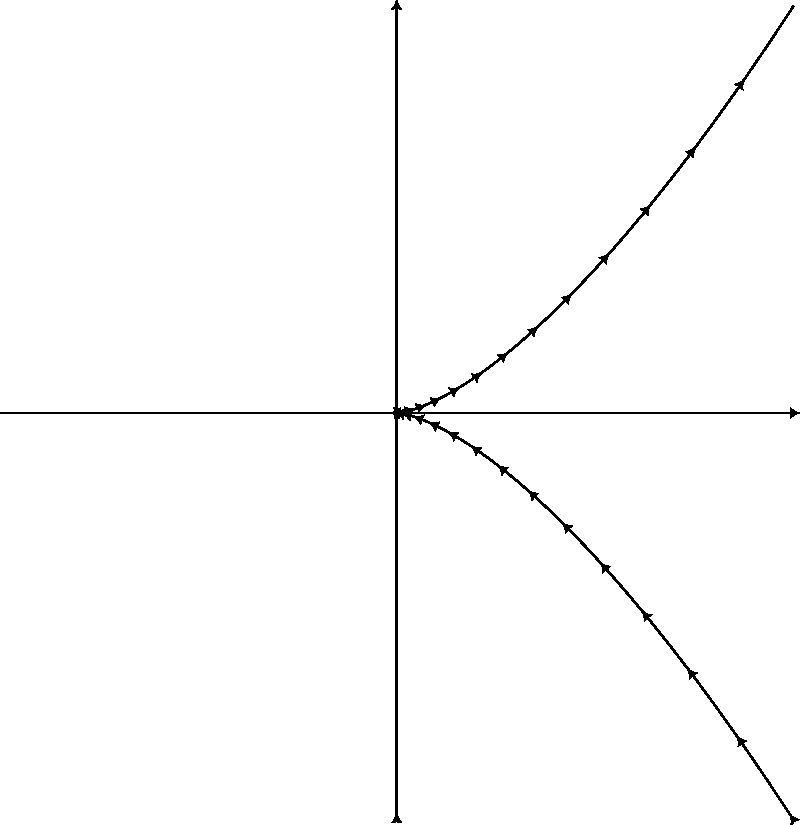
\includegraphics[width=0.5\linewidth]{semicubical_parabola.pdf}
    \end{center}

    $(0,0)$ -- точка излома (т.е. точка, в которой параметризация теряет регулярность).
\end{example}

\subsection{Перепараметризация}
Пусть $\phi: [a,b] \to [c,d]$, $\phi$ строго возрастает, $\phi(a) = c, \phi(b) = d$, также существует $\phi^{-1}$.
$\vf: [c,d] \to \R^3$, тогда $\vg \coloneqq \vf \circ \phi: [a,b] \to \R^3$.
В таком случае $\vg$ -- перепараметризация кривой и $\vf = \vg \circ \phi^{-1}$.

Если такая $\phi$ существует, то $\vf \sim \vg$ (эквивалентны).

Если образы $\vf(t)$ и $\vg(t)$ совпадают, кривые не самопересекаются,
а их параметризации регулярны, то существует такое $\phi$ и $\vf = \vg \circ \phi$.

\section{Длина кривой}
\begin{definition}[Длина кривой]
    $\vf: [a,b] \to \R^3$, $a = t_0 < t_1 < ... < t_n = b$, $\Delta_i t = t_i - t_{i-1}$.
    \[L \coloneqq \lim_{\max \Delta_i t \to 0} \sum_{i=1}^n |\vf(t_i) - \vf(t_{i-1})|\]
\end{definition}

\begin{definition}[Спрямляемая кривая]
    Прямая называется спрямляемой, если существует её длина.
\end{definition}
\begin{example}
    $y = \sin 1/x$  на $(0, 1]$ не спрямляемая.
    \begin{center}
        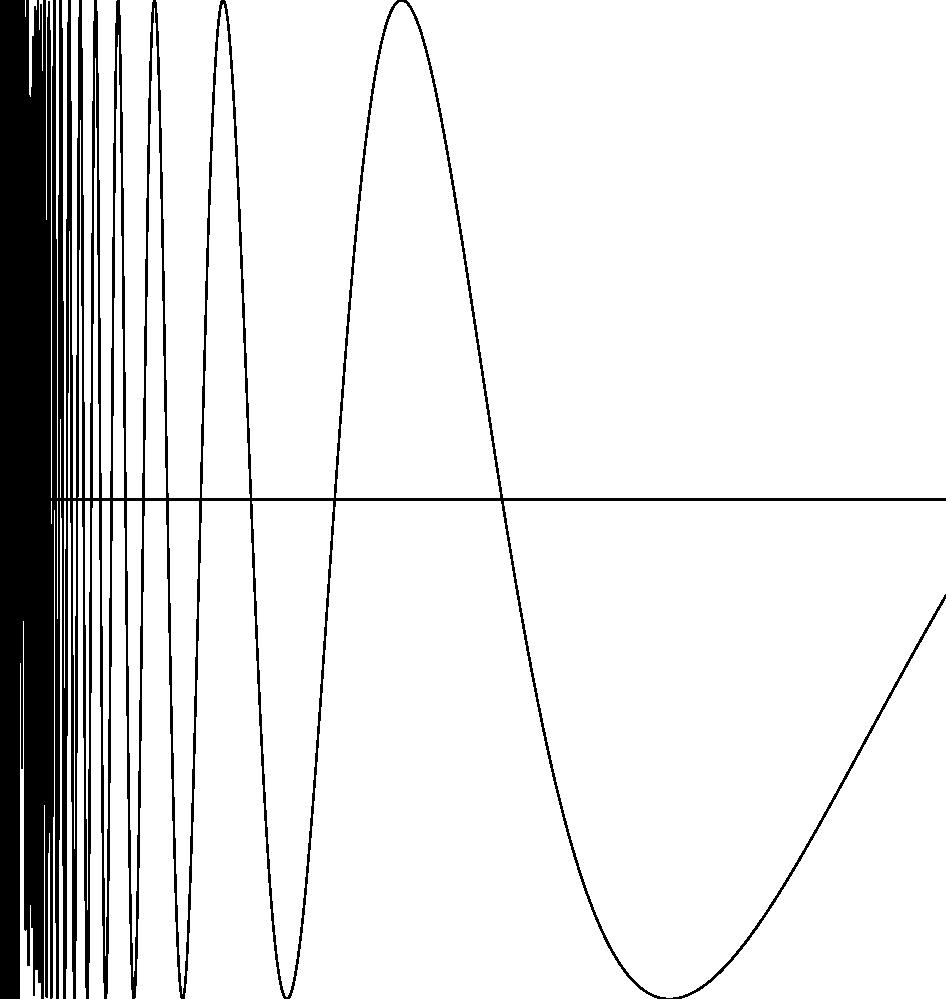
\includegraphics[width=0.5\linewidth]{sin_1_over_x.pdf}
    \end{center}
\end{example}
\begin{example}
    $y = \sqrt{x} \sin 1/x$, $y(0) = 0$, ее сумма оценивается $L \ge \sum_{n=1}^\infty \sqrt{\frac{1}{n}} = \infty$.
\end{example}
\begin{theorem}
    \[L = \int_a^b |\vf'(t)| dt \]
\end{theorem}
\begin{remark}
    $|\sum \vf_i| \le \sum |\vf_i|$, $||\vf| - |\vg|| \le |\vf - \vg|$, $|\int \vf dt| \le \int |\vf| dt$.
\end{remark}
\begin{proof}
    Хотим доказать:
    \[\left| \int_a^b |\vf'(t)| dt - \sum |\vf(t_i) - \vf(t_{i-1})|\right| \to 0\]
    оценим это:
    \begin{multline*}
        \left| \int_a^b |\vf'(t)| dt - \sum |\vf(t_i) - \vf(t_{i-1})|\right| = \\
        \left| \int_a^b |\vf'(t)| dt - \sum |\vf'(\sigma_i)| \Delta_i t  + \sum |\vf' (\sigma_i)| \Delta_i t - \sum |\vf(t_i) - \vf(t_{i-1})| \right| \\
        \le \left| \int_a^b |\vf'(t)| dt - \sum |\vf'(\sigma_i)| \Delta_i t \right|  +\\
        \left| \sum |\vf' (\sigma_i)| \Delta_i t - \sum |\vf(t_i) - \vf(t_{i-1})| \right|
    \end{multline*}
    $\left| \int_a^b |\vf'(t)| dt - \sum |\vf'(\sigma_i)| \Delta_i t \right| \to 0$ по определению интеграла.

    $\vf'$ непрерывная, значит равномерно непрерывна, тогда если
    $\forall \epsilon > 0\  \exists \delta > 0\  |x_1 - x_2| < \delta \implies |\vf(x_1) - \vf(x_2)| < \epsilon$.
    Выберем любое $\epsilon$ и зафиксируем $\delta$, удовлетворяющее мелкости разбиения и получим:
    \begin{multline*}
        \left| \sum |\vf' (\sigma_i)| \Delta_i t - \sum |\vf(t_i) - \vf(t_{i-1})| \right| =\\
        \left|\sum \int_{t_{i-1}}^{t_i} |\vf'(\sigma_i)|dt -  \sum \left|\int_{t_{i-1}}^{t_i} \vf'(t)dt\right|\right|
        \le \sum \int_{t_{i-1}}^{t_i} \left|\vf'(\sigma_i) - \vf'(t) \right|dt \\
        \le \sum \int_{t_{i-1}}^{t_i} \epsilon dt = \epsilon (b-a) \to 0
    \end{multline*}
\end{proof}

\newpage % It's a curse! Remove if something moves before this!
\marginpar{12.09.22}
Попытаемся понять как вычислять длину прямой в некоторых случаях:
\begin{itemize}
    \item в случае явного задания:
          \begin{gather*}
              \displaystyle \begin{cases}
                  x = t \\
                  y = f(t)
              \end{cases} \Leftrightarrow y = f(t) \\
              |(x',y')|  = \sqrt{1 + \vf'^2(t)} \implies
              L = \int_a^b\sqrt{1 + \vf'^2(t)} dt
          \end{gather*}
          К сожалению, такая формула мало применима, так как интегралы берутся редко.
    \item в случае параметрического задания:
          \begin{gather*}\begin{cases}
                  x = x(t) \\
                  y = y(t) \\
                  z = z(t)
              \end{cases} \implies
              L = \int_a^b \sqrt{x'^2 + y'^2 +z'^2} dt
          \end{gather*}
    \item в случае полярных координат:
          \begin{gather*}
              r = r(\phi) \Leftrightarrow \begin{cases}
                  x = r(\phi) \cos \phi \\
                  y = r(\phi) \sin \phi
              \end{cases} \implies
              \begin{cases}
                  x' = r' \cos \phi -r \sin \phi \\
                  y' = r' \sin \phi + r \cos \phi
              \end{cases} \\
              \begin{multlined}
                  x'^2 + y'^2 = (r' \cos \phi -r \sin \phi)^2 + (r' \sin \phi + r \cos \phi)^2 = \\
                  r'^2\cos^2 \phi - 2rr'\sin \phi \cos \phi + r^2 \sin^2 \phi +\\
                  r'^2 \sin^2\phi + 2rr' \sin \phi \cos \phi + r^2 \cos^2 \phi = \\
                  r'^2 + r^2
              \end{multlined}\\
              L = \int_a^b \sqrt{x'^2 + y'^2} d\phi  = \int_a^b \sqrt{r'^2 + r^2}d \phi
          \end{gather*}
\end{itemize}

\section{Касательный вектор}
\begin{lemma}\label{dfoc:very_important_lemma}
    Если $|\vf(t)| = const$, то $\vf'(t) \perp \vf(t)$.
\end{lemma}
\begin{proof}
    Из $\vf'(t) \perp \vf(t)$ получаем: $ (\vf'(t), \vf(t)) = 0\ \forall t$.
    Возьмем производную скалярного квадрата и получим:
    \[(\vf(t), \vf(t))' = 2(\vf'(t), \vf(t)) = 0 = |\vf(t)|^{2'}\]
    Тогда, $|\vf(t)| = const$.
\end{proof}
\begin{definition}[Касательный вектор]
    $\vf'(t_0)$ называется касательным вектором к кривой в точке $t_0$.
    Прямая, на которой лежит $\vf'(t)$ -- касательная прямая.
\end{definition}
\begin{theorem}
    Касательная прямая не зависит от параметризации, если она регулярна.
\end{theorem}
\begin{proof}
    $\phi$ -- скалярная функция, $\vf(t)$ -- вектор-функция.
    Также $\vf(\phi(t)) = \vg(t)$.
    $\vf'(t)$, $\vg'(t) = \vf'(\phi(t)) \phi'(t)$ -- касательные векторы $\vf$ и $\vg$ соответственно.
    Обозначим $\tau = \phi(t)$.
    $\vf'(t)$ и $\vg'(t)$ отличаются друг от друга на скаляр,
    тогда $\vf'(\tau) \parallel \vg'(t)$.
    Следовательно, при перепараметризации касательный вектор будет параллелен предыдущему, значит касательная прямая инвариантно определена.
\end{proof}
\begin{remark}
    Регулярная параметризация -- это параметризации для которой в любой точке существует касательная прямая.
\end{remark}
\begin{definition}[Натуральная параметризация]
    Параметризация $\vf(t)$ называется натуральной, если $|\vf'(t)| \equiv 1\ \forall t$.
\end{definition}
По сути, мы идем по кривой с единичной скоростью.
Но пока не ясно существует и единственна ли натуральная параметризация.
\begin{proof}
    Проверить единственность достаточно просто: $\vg(t) = \vf(\phi(t))$, $\phi(t) = \tau$
    \[|\vg'(t)| = |\vf'(\tau)| |\phi(t)| \implies |\phi'(t)| = 1\]
    тогда $\phi = t + t_0$ (с точностью до выбора начального момента времени).
\end{proof}

\begin{theorem}
    Натуральная параметризация существует.
\end{theorem}
\begin{proof}
    Вспомним про длину кривой.
    Глобальная идея: параметризация говорит сколько мы проходим по кривой за данное время;
    чтобы перейти к натуральной параметризации мы откажемся от стандартного времени,
    и скажем, что новое время это тот участок кривой, за которое мы его проходим, или
    единичное расстояние мы проходим за единичное время, значит параметр времени -- это участок дуги.

    Реализуем эту идею:
    \[s = \int_{t_0}^t |\vf'(\tau)| d\tau\]
    $s$ -- искомый натуральный параметр.
    Будем считать $t - t_0$ временем.
    Обозначим $s = \phi(t)$:
    \[\phi(t) = \int_{t_0}^t |\vf'(\tau)| d\tau\]
    Заметим, что $\phi(t)$ возрастает и непрерывна.
    Значит существует $t = \phi^{-1}(s)  = \psi(s)$.
    Тогда $\vf(t) = \vf(\psi(s))$ должна быть натуральной параметризацией.

    Теперь докажем, что $\vf(\psi(s))$ есть натуральная параметризация.
    Хотим убедиться, что
    \[\left| \frac{d \vf(\psi(s))}{ds}\right| = 1.\]
    Для этого
    \begin{gather*}
        \psi'(s) = \frac{1}{\phi'(t(s))} = \frac{1}{|\vf'(t)|}\\
        \frac{d}{ds}\vf(\psi(s)) = \vf'(\psi(s)) \psi'(s) = \frac{\vf'(t)}{|\vf'(t)|}\\
        \left| \frac{\vf'(t)}{|\vf'(t)|} \right| = 1
    \end{gather*}
\end{proof}

\section{Реп\'ер Френ\'е}

Есть кривая и $\vf(s)$ -- ее натуральная параметризация, тогда $\vv(s)$ -- ее касательный вектор.
$|\vv(s)| = 1$.
Тогда $\vv'(s) \perp \vv(s)$ по лемме \ref{dfoc:very_important_lemma}.
\begin{definition}[Кривизна кривой]
    Определим $\vn(s)$: $\vn(s) \upuparrows \vv'(s)$, $|\vn(s)| = 1$,
    такой $\vn$ -- вектор главной нормали.
    \[k = \frac{\vv ' (s)}{\vn} \Leftrightarrow \vv' = k \vn\]
    Такая $k$ -- кривизна кривой.
    А выражение $\vv' = k \vn$ называется первой формулой Френе.
\end{definition}
\begin{remark}
    $k \ge 0$.
\end{remark}
\begin{remark}
    $\vn$ -- не везде определен, необходима бирегулярность.
\end{remark}

\begin{definition}
    Кривая называется бирегулярной, если $\vf''(t) \not\parallel \vf'(t)$ для любой параметризации.
    Или, если $\vv'(s) \neq 0$ для натуральной параметризации.
    Или $\vn$ корректно определен.
    (почему они эквивалентны -- вопрос будущего)
\end{definition}

По умолчанию считаем, что все кривые бирегулярны.

У нас есть вектор $\vv$ и перпендикулярный ему $\vn$.
Они единичные, хотим превратить их в базис пространства.
Для этого построим вектор $\vb$ перпендикулярный им обоим и тоже единичный.
\begin{center}
    \import{figures/}{binormal_vector.pdf_tex}
\end{center}

\begin{definition}[Вектор бинормали]
    \[\vb \coloneqq \vv \times \vn\]
    Правая тройка $(\vv,\vn, \vb$) -- репер Френе.
\end{definition}

Изучим $\vb'$:
$\vb'(s) \perp \vb(s)$ из леммы \ref{dfoc:very_important_lemma},
также $\vb' \perp \vv$. Почему?
\[\vb' = (\vv \times \vn)' = \vv' \times \vn + \vv\times \vn' = 0 + \vv\times \vn' \perp \vv\]
Таким образом, $\vb' \parallel \vn$ и $\vb' = -\kappa \vn$ -- вторая формула Френе.
\begin{definition}[Кручение кривой]
    $\kappa$, определенная выше -- кручение кривой.
\end{definition}

Изучим $\vn$:
\[\vn' = (\vb \times \vv)' = \vb' \times \vv + \vb \times \vv' = -\kappa \vn \times \vv + \vb \times k\vn = \kappa\vb - k\vv\]
получили третью формулу Френе.
\begin{definition}[Формулы Френе]
    \[
        \begin{array}{cccc}
            \toprule
                 & \vv & \vn     & \vb    \\ \midrule
            \vv' & 0   & k       & 0      \\ \midrule
            \vn' & -k  & 0       & \kappa \\ \midrule
            \vb' & 0   & -\kappa & 0      \\
            \bottomrule
        \end{array}
    \]
    Производная везде берется по натуральному параметру.
\end{definition}
\begin{definition}
    Плоскость $(\vn, \vb)$ -- нормальная плоскость кривой.
    Плоскость $(\vv, \vn)$ -- соприкасающаяся плоскость кривой.
    Плоскость $(\vv, \vb)$ -- спрямляющая плоскость кривой.
\end{definition}

Вопрос: а как это посчитать?
\begin{example}
    Есть окружность:
    \[\begin{cases}
            x = R \cos t \\
            y = R \sin t \\
            z = 0
        \end{cases}\]
    Хотим найти натуральную параметризацию:
    сейчас мы проходим окружность за время $2\pi$, наверное нужно проходить окружность за время $2\pi R$.
    Тогда получим:
    \[\begin{cases}
            x = R\cos (t/R)  \\
            y = R \sin (t/R) \\
            z = 0
        \end{cases}
        \implies
        \begin{cases}
            x' = - \sin (t/R) \\
            y' = \cos (t/R)
        \end{cases}\]
\end{example}
\end{document}